\articlehead{Furry Art in Depth}{Zik}{2012}

When a non-fur asks for an example of what the ``furry fandom'' is, you show them convention websites or furry social sites. When a non-fur asks what a furry is, you show them a picture of an anthropomorphic animal. The most integral and fundamental part of the fandom is its artwork. Furry artwork serves many purposes within the fandom, and for every purpose there are artists focused on that form of design. Convention posters, story illustrations, popular media, and personal art, both custom and non-custom, are just some of the uses for which ``furry'' artwork is created.

Within the realm of personal anthropomorphic pics, there are plenty of ways to acquire your own artwork.  All you have to do is consider what sort of art you're interested in, where it will be shown, and a budget. Most furries nosing around the art-o-sphere are searching for custom commissions. They can start by considering whether they're looking for traditional or digital art. Traditional art is created with physical media like colored pencils, watercolors, and even oil paint. Digital art is created using any number of the digital art suites available on the Internet.

There's a separation between two different kinds of artistic production: functional and aesthetic. The distinction is more important than the fandom might consider. In order to explore this idea, let me give a quick run-down on the history of creative art during arguably the most important artistic era of all time: the Renaissance.

In pre-Renaissance Italy ``artists'' as we know of it were virtually unheard of. The creators of ``art'' were artisans, members of a low social class. Artisans were purely craftsmen. They were highly skilled and experienced in their work, which was either functional or decorative: furniture, jewelry, tools, and the like. As a sort of retaliation from the stagnation during the dark ages, painters and sculptors began gaining social status as the general populace finally gained the ability to fund art for their own use. A scientific examination of artistic creation flourished during this time, as optics, geometry, and anatomy were all explored, and ``art'' finally became an intellectual, theoretical practice.

As a result of the new-found esteem of art for art's sake, the upper class of Renaissance Italy began funding portraits as a show of their wealth and nobility. The Catholic Church was also a heavy patron of art in this era, notably the work of Michelangelo. Finally, artists and artisans were a separate group. Those who were skilled in smaller, functional work were a different social class than those who were creating aesthetic pieces for a higher nobility.

\begin{figure}
  \begin{center}
    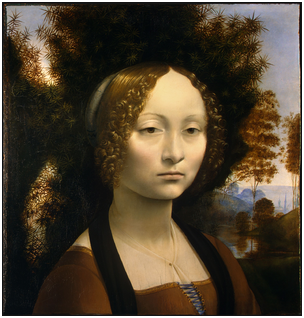
\includegraphics{content/assets/furry-art--ginevra}
  \end{center}
  \caption{Ginevra de' Benci``Ginevra de' Benci'' by Leonardo da Vinci, c. 1474.15 x 15 inches, oil on panel. Ginevra was an intelligent aristocrat born in Florence in 1458.}
\end{figure}

Why the historical ramble? The results of the artist/artisan divide echoes in the furry fandom. Consider what function furry artwork fulfills. Badges seem to be the best example of functional artwork. Every badge is a new work, in its own right, but they're generally smaller and less intricate than what one would consider an art piece. They're also geared towards utility: they're something you use to identify yourself in a crowd.

Conventions prominently feature work commissioned from individuals for promotion. Posters, convention book covers, fliers, even custom name tags have been created for conventions as both decoration and to serve a purpose. Some conventions even have mascots which are drawn by new artists each year. Custom t-shirt designs are created for many larger cons. Reference sheets are also significantly functional. While they commonly express a good artistic pose and view or two of a single character, they are above all designed to give viewers a better idea of the character.

As a contrast, consider personal artistic commissions. While badges are usually from \$5-\$30, digital commissions can go upwards of \$100. In addition, physical sketches and original works can cost up to hundreds of dollars. Custom commissions of physical media have run just as high. ``Furry'' has also branched out into the world of actual crafts. A quick lap around the furry marketplace will yield tons of creative craftwork: tails, ears, hats and accessories, embroidery, plushies, even custom pottery. Many furries are finding innovative ways to use different crafts to express animal anthropomorphism.

\begin{figure}
  \begin{center}
    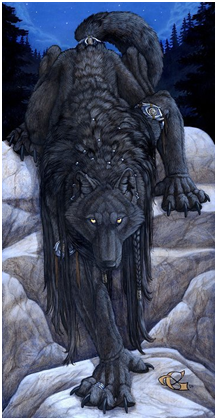
\includegraphics{content/assets/furry-art--eyesofthenight}
  \end{center}
  \caption{Eyes of the Night``Eyes of the Night'' by GoldenWolfen. 22 x 40 inches, acrylic on illustration board. Sold at auction at Further Confusion in 2004 for \$10,000. Said to be the highest selling furry media in the fandom to date.}
\end{figure}

As an artist, you have to consider the same question writers consider: Who is my audience? Or, better yet, a more philosophical: ``Why am I creating this?'' The furry consumer, so to speak, will often settle into a creative need on their own. A badge to use at conventions? A reference sheet to use in roleplay? A tasteful piece to hang in your living room? A motif you want to see your character interacting with? The consumer comes up with an idea. This translates to a need, and the artist has to consider what sort of consumer need they'll be working towards.

Are all furry artists created equal? Not necessarily. Some will create valuable and intricate artwork that takes dozens of hours and some will create simple doodles. All is labeled ``art'', and all creators are labeled ``artists''. However, for the sake of our own insight, consideration of the ``artisan'' might still be relevant. It adds to our understanding of the furry art dynamic. The end result of the Renaissance art movement is a great model for how furries create arts and crafts today.
